% Template for ICASSP-2018 paper; to be used with:
 %          spconf.sty  - ICASSP/ICIP LaTeX style file, and
 %          IEEEbib.bst - IEEE bibliography style file.
 % --------------------------------------------------------------------------
 \documentclass{article}
 \usepackage[latin1]{inputenc}
 \usepackage[T1]{fontenc} 
 \usepackage{spconf,amsmath,graphicx,euler,amsbsy}
 %\usepackage[mathscr]{eucal}
 % Commande de correc à affiner
 \newcommand{\rev}[1]{{\color{black}#1}}
 \newcommand{\modif}[1]{{\color{black}#1}}
 \newcommand{\modifR}[1]{{\color{black}#1}}
 \newcommand{\revv}[1]{{\color{black}#1}}
 \usepackage{algorithm}
\usepackage{algorithmic}
\usepackage{hyperref}
\usepackage{amssymb}

\usepackage[american]{babel}
\usepackage[nopar]{lipsum}
\usepackage{microtype}
\hfuzz=7pt
\hbadness=99999
 % Example definitions.
 % --------------------
 % utils
 \def\F{{\mathcal F}}
 % list of tensor used  in text
 \def\tA{\boldsymbol{{\mathscr A}}}
 \def\tX{\boldsymbol{{\mathscr X}}}
 \def\tY{\boldsymbol{{\mathscr Y}}}
 \def\tG{\boldsymbol{{\mathscr G}}}
 \def\tC{\boldsymbol{{\mathscr C}}}
 % list of matrix used in text
 \def\A{{\mathbf A}}
 \def\S{{\mathbf S}}
 \def\D{{\mathbf D}}
 \def\W{{\mathbf W}}
 \def\H{{\mathbf H}}
 \def\B{{\mathbf B}}
 \def\X{{\mathbf X}}
 \def\G{{\mathbf G}}
 \def\C{{\mathbf C}}
 \def\x{{\mathbf x}}
 \def\y{{\mathbf y}}
 \def\g{{\mathbf g}}
 
% Title.
% ------
\title{Overcomplete Nonnegative Tensor Dictionary Learning (ONTDL) }
%
% Single address.
% ---------------
\name{Author(s) Name(s)\thanks{Thanks to DAISY Normandy region for funding.}}
\address{Author Affiliation(s)}
%
% For example:
% ------------
%\address{School\\
%	Department\\
%	Address}
%
 % Two addresses (uncomment and modify for two-address case).
 % ----------------------------------------------------------
 %\twoauthors
 %  {A. Author-one, B. Author-two\sthanks{Thanks to XYZ agency for funding.}}
 %	{School A-B\\
 %	Department A-B\\
 %	Address A-B}
 %  {C. Author-three, D. Author-four\sthanks{The fourth author performed the work
 %	while at ...}}
 %	{School C-D\\
 %	Department C-D\\
 %	Address C-D}
 %

\begin{document}

 %\ninept
 %
 \maketitle
 %
 \begin{abstract}
 Sparse coding, that is, modelling data vectors as sparse linear combinations of basis elements, is widely used in neuroscience, signal processing, etc.... Sparse coding in Time-Frequency (TF) domain is generally performed through Nonnegative Matrix Factorization (NMF) with  sparsity penalty with application in several tasks such as image denoising \cite{refDictionaryImagedenoising}. 
 One of the main drawbacks of the NMF is that for some classes of signals (e.g signal presenting spectral patterns modulated in time ), it  cannot directly take into account temporal patterns, in the sense that it cannot be done  without large number of basis elements and a post-processing step to group the basis elements into single events. In order to circumvent of this drawback, we propose a tensor-based dictionary learning approach. A proof of concept performed on synthetic data set proves the ability of our approach to better take into account temporal patterns compared to NMF.
 \end{abstract}
 \begin{keywords}
Tensors, dictionary learning, Spectrogram, Nonnegative Matrix Factorization(NMF), spectral patterns, temporal patterns.
 \end{keywords}
 %
 \section{Introduction}
 \label{sec:intro} 
 %POSSIBLE  here!!!!!!(PRESENT THE AUDIO SCENE CLASSIFICATION PROBLEM)
 
%CURRENT METHODS: the features used: MFCC or Spectrogram (use the article casadeep AR).
%Methods: deep-based and no deep
%(I make the reader notice that I am aware of the existence of deep-based methods)


%No deep methods: try to extract frequency PATTERNS relevant to each class: each audio scene (images) decomposes in term of (check the verb decompose) a small number of elementary atoms containing these frequency patterns and activation coefficients(to check) describing which atoms are present and when. Recovering simultaneously the atoms and the activation coefficients is called ''Dictionary Learning'' problem.

%However, there are some classes of signals for which standard NMF would require to use a large number of bases, and some postprocessing
%to group the bases into single events. This is in particular what happens when we deal with a signal presenting spectral patterns modulated in time while its variations
%in time are actually much richer.

%This is in particular what happens when we deal with a signal presenting spectral patterns modulated in time.
%(shingle: read, understand and put there a sentence).
Audio scene classification is a complex problem
which aims at recognizing acoustic environments
solely based on an audio recording of the scene. Most works
have focused on investigating discriminative representations
for audio acoustic scenes, the most used being MFCC and Time-Frequency (TF) representation from which some hand-crafted features are derived such as recurrence quantitative analysis (RQA)\cite{refRQA}, Deep Neural Networks (DNN)\cite{refDNN},etc...
\\
Deep neural networks model generally need large amounts of data and extensive computations\cite{Deepproblem} and are not easily interpretable. A good alternative to these restrictions may be matrix processing.
\\
When dealing with spectrograms, some of the  classical methods that do not resort to neural networks try to extract \textbf{frequency patterns} relevant to each signal by decomposing the signals in term of a small number of elementary atoms containing these frequency patterns and activation coefficients describing which atoms are present in a given signal. Recovering simultaneously the atoms and the activation coefficients is called \textbf{Dictionary Learning} problem.
Several frameworks have been proposed to perform this decomposition. When positivity is inherent to the data (e.g spectrogram ), this task can be performed by Nonnegative Matrix Factorization with sparsity penalty enabling the presence of redundant atoms. The activation coefficients associated to each scene are then used as the inputs of a classifier.
\\
One of the main drawback of this technique is that \textbf{temporal patterns} are not directly taken into account during the decomposition step. Precisely, NMF would require to use a large number of basis elements, and a  post-processing step
to group them into single events when dealing with a signal presenting spectral patterns modulated in time  while its variations
in time are actually much richer \cite{ProblemNMF}.
To circumvent this drawback, we propose a nonnegative dictionary learning approach based on tensor representation. The main idea is to approximate a three order tensor by the product of a tensor representing activation coefficients, a matrix of spectral atoms and a matrix of temporal atoms which model the temporal patterns while giving the possibility to have overcompleteness. We hope for example that the temporal atoms would help us to better discriminate two signals with the same spectral patterns (e.g low frequencies) with different lengths in time.
While the relationship between Multimodal dictionary learning and tensor decomposition ( either Tucker or Canonical Polyadic Decomposition (CPD)) have been investigated before (\cite{OtherrefDictionaryImagedenoising},\cite{refTuckerChicochi},\cite{CPDictionary}), the previous approaches have been limited  either by reliance on tensor decomposition techniques which  limit the number of dictionary atoms (hence prevent overcompleteness) in Tucker case or by the fact the value of the rank which is not known in general for CPD. Moreover, we impose \textbf{positivity constraints} on the factors inferred by our framework.
A proof of concept performed on synthetic and real data sets proves the ability of the proposed approach to deal with signals presenting frequencies with different temporal patterns compared to NMF.
The rest of the paper is organized as follows. 
%In Section II, the basic notations and brief introduction to tensors are introduced. In section III, the principle of NMF is briefly presented. In section IV, we present our model and provide an algorithm. The following section is devoted to the comparison with state of the arts NMF algorithms.
\section{Tensors and multilinear algebra basics}
A tensor is a multidimensional array defined on the outer product of some vector spaces, the number of vector spaces being the order. Tensors are frequently used today in machine learning and signal processing. The two most commonly used decompositions of tensors are the Tucker and the Parafac models. Given a tensor $\tX\in \mathbb{R}^{\text{I}_{1}\times...\times I_{N}}$, the Tucker model reads:
$\tX \approx \tG \times_{1}\A^{(1)}\times....\times_{N}\A^{(N)}$, $\tG \in \mathbb{R}^{J_{1}\times.....\times J_{N}},\A \in \mathbb{R}^{I_{n}\times J_{n}},J_{n}\leq I_{n}$. The tensor $\tG$ is called the core tensor and the matrices $\A^{(n)}$ are the loading matrices. The canonical model is a special case of Tucker model where each modality of the core tensor is the same, i.e: $J_{i}=J_{j}\forall i,j$ and $\tG_{j_{1},..,j_{N}}\neq 0 $ iff $j_{1}=..=j_{N}$.
In the sequel, we adopt the following notations: the tensors  are denoted by boldface Euler script letters, e.g., $\tX$. The entries of a N-order tensor $\tX\in\mathbb{R}^{I_{1}\times..\times I_{N}}$ are denoted by $\tX_{i_{1},..,i_{N}}$ and the mode-n $(1\leq n\leq N)$ matricized form denoted by $\X^{(n)}$ is a matrix in $\mathbb{R}^{I_{n}\times \prod_{k\neq n}I_{k}}$ defined (according to the reverse lexicographical order) by: $\X^{(n)}_{i,j}=\tX_{i_{1},..,i_{N}}$ with $j=1+\sum^{I_{n}}_{k=1,k\neq n}\prod^{k-1}_{k\neq n}I_{k}$. The mode-n product of $\tX$ with a matrix $\B^{(n)}\in\mathbb{R}^{J_{n}\times I_{n}}$ denoted $\tX\times_{n}\B^{(n)}$yields a tensor $\tY\in \mathbb{R}^{I_{1}\times..\times I_{n-1}\times J_{n}\times I_{n+1}..\times I_{N}}$ defined by:$\tY_{i_{1},.,i_{n-1},j_{n},i_{n+1},.,i_{N}}=\sum^{I_{n}}_{i_{n}=1}\tX_{i_{1},.,i_{n},.,i_{N}}\B^{(n)}_{j_{n},i_{n}}$. Vectors are denoted by boldface lowercase letters, e.g., $\mathbf{a}$. Matrices are denoted by boldface capital letters, e.g., $\A$. Scalars are denoted by lowercase letters, e.g., $a$.The vectorization operator is denoted  $\textbf{Vec}$. For a three-order tensor $\tX \in \mathbb{R}^{K\times I\times J}$, the $\text{k}^{th}$ horizontal slice is the matrix $\tX_{k,:,:}$ obtained by fixed but two indices.
The Frobenius (respectively L1) norm for both matrices and tensors will be denoted as $\|\cdot\|_{F}$ (respectively$\|\cdot\|_{1}$) and defined by:$\|\tX\|^{2}_{F}=\sum_{i_{1},..,i_{N}}\tX^{2}_{i_{1},..,i_{N}}$ ($\|\tX\|^{2}_{F}=\sum_{i_{1},..,i_{N}}|\tX_{i_{1},..,i_{N}}|$). The same  definition holds for matrices. The euclidean norm of a vector $\mathbf{a}\in \mathbb{R}^{N}$ denoted $\|\cdot\|_{2}$ is defined by: $\|\mathbf{a}\|^{2}_{2}=\sum^{N}_{i=1}\mathbf{a}^{2}_{i}$.
\section{Tensor-based model}
\subsection{Nonnegative Matrix Factorization model}
 Given an $K\times L$ nonnegative $\S$ matrix and an integer $K_{d}$ such that   $K\times K_{d}+K_{d}\times L\ll K\times L$, NMF approximates $\S$ by the product of an $K\times K_{d}$ matrix $\W$ and an $K_{d}\times L$ matrix $\H$, i.e:$\S \approx \W\H$. 
 This decomposition is generally performed by minimizing a cost function $\mathbb{C}(\W,\H)$ with respect to $\W$ and $\H$. 
 The usual divergence measures are the Euclidean divergence,Kullback Liebler divergence
and Itakura Saito divergence. When applied to power spectrogram, NMF factorizes data into a basis of frequency templates and a matrix of temporal activation vectors. NMF is able to project all signals that have the same spectral shape on a single basis, which allow to represent a variety of phenomena efficiently using a very compact set of basis elements. However, since NMF is originally a dimensionality reduction technique, a lot of information can be lost. This lost can be enhanced when dealing with a signal presenting spectral patterns whose amplitude
are modulated in time. Learning dictionary atoms with such time-varying spectra through
standard NMF would require to use a large number of basis elements, and a post processing step to group them into single events.
To try to alleviate the extent of this drawback, we present a tensor-based dictionary learning framework.
\subsection{Overcomplete Nonnegative Tensor Dictionary Learning (ONTDL)}
Let's consider a three order tensor $\tX$ whose horizontal slices represent spectrograms $\left\{S\right\}_{1\leq k\leq K}$ of K signals (each spectrogram being in $\mathbb{R}^{I_{f}\times I_{t}}$). Our model approximates the tensor $\tX\in \mathbb{R}^{K\times I_{f}\times I_{t}}$ by the product of activation coefficients ($\tG\in\mathbb{R}^{K\times J_{f} \times J_{t}}$) with a matrix whose columns represent spectral patterns $\A^{(f)}\in\mathbb{R}^{I_{f}\times J_{f}}$ and a matrix whose columns embody temporal patterns $\A^{(t)}\in\mathbb{R}^{I_{t}\times J_{t}}$, i.e: $\tX \approx\tG\times_{1}I\times_{2}\A^{(f)}\times_{3}\A^{(t)}$. 
. It is not difficult to see that this corresponds to a dictionary learning framework. One simple way to notice it is the following one: it is straightforward to see that $\tX_{k,:,:}\approx \sum_{i,j|\tG_{k,i,j}\neq 0}\tG_{k,i,j}\A^{(f)}_{:,i}o\A^{(t)}_{:,j}$(o being outer product). This means the $k^{th}$ spectrogram is a linear combination of some basis images $\A^{(f)}_{:,i}o\A^{(t)}_{:,j}$. Hence, the coefficients $\tG_{k,i,j}$ represent activation coefficients associated to the $k^{th}$ spectrogram. Besides, it is quite easy to see that:$Vec(\tX_{k,:,:})\approx (\A^{(f)}\otimes \A^{(t)})Vec(\tG_{k,:,:})$. Since $\tG_{k,:,:}$ represent activation coefficients, $\A^{(f)}$ and $\A^{(t)}$ represent spectral and dictionary atoms.
\textbf{Even though it is very similar to the Tucker decomposition, it differs from the classical Tucker decomposition which imposes $I_{f}\geq J_{f},I_{t}\geq J_{t}$.  We lift this restrictions in our framework, which paves the way to overcomplete dictionary learning: if $I_{f}< J_{f}$ and $I_{t}<J_{t}$,  $\underbrace {I_{f}\times I_{t}}_{\text{signal dimension}}<\underbrace{J_{f}\times J_{t}}_{\text{number of dictionaries}}$}, which corresponds to the definition of redundant dictionaries\\
In order to infer $\tG,\A^{(f)},\A^{(t)}$, we propose to solve the
following problem:\\
$\min \underbrace{ \mathcal{F}(\tG,\A^{(f)},\A^{(t)})}_{\text{Fidelity term}}+\lambda_{info} \underbrace{\xi(\tG,\B^{(f)},\B^{(t)})}_{\text{Penalty}}+\lambda_{g}\|\tG\|_{1}$\\
w.r.t $\tG,\A^{(f)},\A^{(f)},\B^{(f)},\B^{(t)}\geq 0,\|\A^{(f)}\|^{2}_{F}\leq 1,\|\A^{(t)}\|^{2}_{F}\leq 1,\|\B^{(f)}\|^{2}_{F}\leq 1,\|\B^{(t)}\|^{2}_{F}\leq 1$.\\
The term $\xi$ is used to incorporate class information in the minimization process and then paves the way to a supervised framework. It can be easily dropped out to solve the problem in an unsupervised way and this will not change anything to the reasoning and obviously, the class penalty term can be easily replaced by any kind of class information penalty\cite{ExampleofSupervisedTucker}\\
In the sequel, we will use Euclidean divergence for the fidelity term (aims at reconstructing each signal as positive linear combination of spectral and temporal dictionaries) and class penalty (which is designed to make the activation coefficients aligned with an information tensor), ie:\\
$\mathcal{F}(\tG,\A^{(f)},\A^{(t)})=\|\tX -\tG\times_{1}I\times_{2}\A^{(f)}\times_{3}\A^{(t)}\|^{2}_{F}$
\\
$\xi(\tG,\B^{(f)},\B^{(t)})=\| \tC - \tG \times_1 I \times_2 \B^{(f)} \times_3 \B^{(t)} \|_{F}^2$,
\\
$\tC_{k,i,j}=\mathbf{1}_{[(c_{k}-1)\frac{J_{f}}{M},c_{k}\frac{J_{f}}{M}]\times [(c_{k}-1)\frac{J_{t}}{M},c_{k}\frac{J_{t}}{M}]}(i,j)$ with:
\\
$\mathbf{1}_{A\times B}(i,j)=1$ if $i\in A$ and $j\in B$, 0 otherwise,$c_{k}$ the label associated to the $k^{th}$ example. We assume that $J_{f}$ and $J_{t}$ are divisible by M, M being the number of classes.\\
The third term is used to enforce sparsity on the core tensor. The $L_{2}$ penalty is intended to prevent the core tensor entries from being too large.\\
We adopt the classical approach to solve this class of problems which is about associating penalty terms to the constraints:\\
$\min \mathcal{F}(\tG,\A^{(f)},\A^{(t)}) +\lambda_{info}\xi(\tG,\B^{(f)},\B^{(t)})  +\lambda_{g}\|\mathcal{G}\|_{1}+\frac{\alpha(1-\theta)}{2}\|\A^{(f)}\|^{2}_{F}+\frac{\alpha(1-\theta)}{2}\|\A^{(t)}\|^{2}_{F}+\frac{\alpha(1-\theta)}{2}\|\B^{(f)}\|^{2}_{F}+\\\frac{\alpha(1-\theta)}{2}\|\B^{(t)}\|^{2}_{F}$\\
w.r.t $\tG,\A^{(f)},\A^{(t)},\B^{(f)} ,\B^{(t)}\geq 0$.\\
In the sequel, we denote this objective function by\\ $\Gamma(\tG,\A^{(f)},\A^{(t)},\B^{(f)},\B^{(t)})$ in the sequel.\\
Since there is no analytical solution, we solve the problem by an alternating minimization scheme whose framework is as follows (see Appendix for more details about the different updates):
\begin{algorithm}[H]
\caption{Perform the ONTDL}
%\KwIn{ 
\textbf{Inputs}:$\tX$ : the tensor of interest,
Coretensorsize : the desired size of the core tensor,
nbclasses:the number of classes,$\mathcal{C}$: the information tensor.
\\
\textbf{Outputs}: the loading matrices $\A^{(f)}$, $\A^{(t)}$ and the core tensor $\tG$
\\
\textbf{Initialization}:$k=0,\A^{(f)}_{k},\A^{(t)}_{k},\B^{(f)}_{k},\B_{k}^{(f)},\tG_{k}$

\begin{algorithmic}
\WHILE{a stopping condition is verified}{
 \STATE $\tG_{k+1}=argmin_{\tG\geq 0}\Gamma(\tG,\A^{(f)}_{k},\A^{(t)}_{k},\B^{(f)}_{k},\B^{(t)}_{k})$
 \STATE $\A^{(f)}_{k+1}=argmin_{\A\geq0}\Gamma(\tG_{k+1},\A,\A^{(t)}_{k},\B^{(f)}_{k},\B^{(t)}_{k})$
 
 \STATE $\A^{(t)}_{k+1}=argmin_{\A\geq0}\Gamma(\tG_{k+1},\A^{(f)}_{k+1},\A,\B^{(f)}_{k},\B^{(t)}_{k})$ 
 
 \STATE $\B^{(f)}_{k+1}=argmin_{\B\geq0}\Gamma(\tG_{k+1},\A^{(f)}_{k+1},\A^{(t)}_{k+1},\B,\B^{(t)}_{k})$ 
 \STATE $\B^{(t)}_{k+1}=argmin_{\B\geq0}\Gamma(\tG_{k+1},\A^{(f)}_{k+1},\A^{(t)}_{k+1},\B^{(f)}_{k+1},\B)$ \\
   }  
\ENDWHILE
\end{algorithmic}
\end{algorithm}
\section{Experiment}
In these experiments, we compare our approach to two supervised NMF problems on synthetic and real data sets. The objective is not about achieving state of arts performance on the real data set,but to prove that temporal patterns can improve our ability to discriminate in a classification framework.
\subsection{Experimental setup}
We define a 3-order tensor $\tX$ whose frontal slices represent the spectrograms $S_{k}$ of the training examples.
We extract  both training and test features by projecting the spectrograms on temporal dictionaries $\A^{(t)}_{s}$ and spectral dictionaries $\A^{(f)}_{s}$ inferred by ONTDL applied to $\tX$,i.e:\\
$Feature_{k}\leftarrow argmin_{G\in \mathbb{R}^{J_{f}\times J_{t}},G\geq 0}\|\S_{k}-\A^{(f)}_{s}G\A^{(t)T}_{s}\|^{2}_{F}+\theta\alpha\|G\|_{1}$, 
$Feature_{k}$ being the example associated to the $k^{th}$ signal. We compare ONTDL to the  dictionary learning NMF-based approach. We compare our approach to two NMF problems:\\
$\min\|\S-\D\A\|^{2}_{F}+\lambda_{info}\|\C-\X\A\|^{2}_{F}+\alpha\theta\|\A\|_{1}$w.r.t $\D,\A,\X\geq 0$,$(\mathcal{P}_{1})$\\
$\min\|\S-\D\A\|^{2}_{F}+\lambda_{info}\|\C-\X\A\|^{2}_{F}+\alpha\theta\|\A\|_{1}+\frac{(1-\theta)\alpha}{2}\|\D\|^{2}_{F}+\frac{(1-\theta)\alpha}{2}\|\X\|^{2}_{F}$,w.r.t $\D,\A,\X\geq 0$,$(\mathcal{P}_{2})$.\\
The problem $\mathcal{P}_{1}$ is the classical sparse coding problem in which we incorporate a class information penalty and the problem $(\mathcal{P}_{2})$ is derived from ($\mathcal{P}_{1})$ by imposing constraints on the coefficients of $\D$ and $\X$ in order to prevent the coefficients of $\A$ from being too large, which is also an approach encountered in sparse coding.\\ 
The matrix $S$ and $C$ are defined by:
$S=[\S_{1},...,\S_{N}]$,\\
$\C_{i,j}=1$ if $i\in [(c-1)\frac{Kd}{M}+1,c\frac{Kd}{M}]$ and the $j^{th}$ signal belongs to class c and 0 otherwise.Kd is the number of dictionary atoms and is assumed to be a multiple of the number of classes M. It is worth to notice that that this matrix $\C$ and the associated penalty have already been proposed in \cite{Classinformation}. We use two different approaches to solve this problem: projected gradient(this method will be referred to as DLPG and is performed by the algorithm presented in \cite{PGD} and available on scikitlearn) for the problem $(\mathcal{P}_{1})$ and
coordinate descent (this method will be referred to as DLCD and is performed by the algorithm presented in \cite{FCD} and available on scikitlearn) for the problem $(\mathcal{P}_{2})$. The training and test features are computed by projecting the spectrograms on the dictionary D:
$Feature_{k}\leftarrow argmin_{\A\geq 0}\|\S_{k}-\D\A\|^{2}_{F}+\theta\alpha\|\A\|_{1}$,$Feature_{k}$ being the feature associated to the $k^{th}$ example. 
The performance criterion is the mean average precision:
$MAP=\frac{1}{N}\sum^{N}_{i=1}PWC_{i}$; $PWC_{i}$: proportion of well classified examples in $i^{th}$ class,N: the number of classes. For each experiment, we use a SVM classifier with the parameter C and $\sigma$ chosen by cross validation. The linear regression problems related to each to each feature extraction process are solved by the tool made available by 
\subsection{Synthetic data}
We consider a simulated data set composed of 400 samples split into 8 classes (50 samples per class). The 8 classes are composed of signals $s_{\beta_{1},\beta_{2},\alpha_{1},\alpha_{2},\theta}(t)=s^{\beta_{1},\beta_{2}}_{1}(t)+s^{\alpha_{1},\alpha_{2}}_{2}(t)$ defined by:
\\
$s^{\beta_{1},\beta_{2}}_{1}(t)=\mathbf{1}_{[t_{0}+\beta_{1},t_{1}+\beta_{2}]}(t)cos(2\pi\times f_{\theta}(t))$
\\
$s^{\alpha_{1},\alpha_{2}}_{2}(t)=\mathbf{1}_{[t_{0}-\alpha_{1},t_{1}-\alpha_{2}]}(t)cos(2\pi\times f_{\theta}(t))$
\\
$f_{\theta}(t)=\theta\times(\alpha t+\beta)\times t$.\\
t refers to the time and $f_{\theta}$ the frequency. The values of the parameters $\alpha$ and $\beta$ are respectively fixed to  $\alpha=-1200$ and $\beta=2400$
From the signals $s_{\beta_{1},\beta_{2},\alpha_{1},\alpha_{2},\theta}$, we build a synthetic data set composed of 400 samples split into 8 classes (50 samples per class).For the first four classes, $\theta=2$ and the quadruplets $\left\{\beta_{1},\beta_{2},\alpha_{1},\alpha_{2}\right\}$ associated are respectively:\\
$\text{First class}:\left\{t_{0}+\frac{3}{2},t_{1}+\frac{3}{2},t_{0}-\frac{1}{3},t_{1}-\frac{1}{3}\right\}$,\\
$\text{Second class}:\left\{t_{0}+\frac{3}{2},t_{1}+3,t_{0}-\frac{1}{3},t_{1}-\frac{1}{3}\right\}$,\\
$\text{Third class}:\left\{t_{0}+\frac{3}{2},t_{1}+\frac{3}{2},t_{0}-\frac{1}{3},t_{1}-\frac{1}{300}\right\}$\\
$\text{Fourth class:}:\left\{t_{0}+\frac{3}{2},t_{1}+3   ,t_{0}-\frac{1}{3},t_{1}-\frac{1}{300}\right\}$\\
The signals of fifth, sixth, seventh and eighth classes are respectively defined as the first, second, third and fourth signals by fixing $\theta$ to 5.5. We apply the framework presented in the previous section to $\tX_{n}$ defined as follows:\\
$\tX_{n}=\tX_{train}+\mathcal{U}$, with $\mathcal{U}$ with: $\tX_{train}$ containing the spectrograms of the training examples and $\mathcal{U}$ being a random variable whose elements are drawn from a uniform  on $[0,20]$. For dimensionality purpose, we resize the spectrograms by cubic interpolation to $30\times 30$ images. The paramter C and $\sigma$ are selected among 4 values logarithmically scaled between $10^{-3}$ and $10^{-8}$. The values of $\alpha,\theta,\lambda_{info},\lambda_{g}$ are respectively fixed to $10^{-4},10^{-3},10^{-4},10^{-4}$,. The features extraction is performed according to the experimental setup and the average classification performance over 5 different noises for different numbers of training examples is given by the following chart:

\begin{figure}[!ht]
\centering
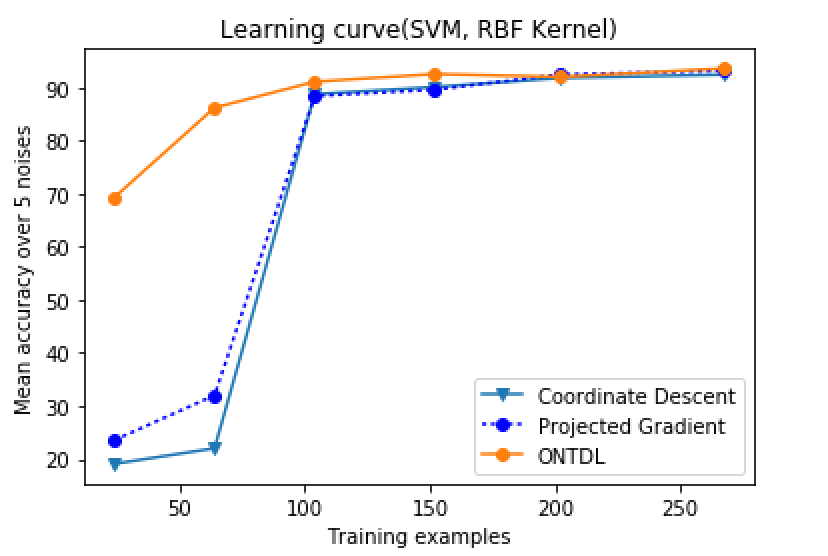
\includegraphics[width=4.5cm]{LearningCurveToy.png}
\caption{Learning curve:32 spectral dictionary atoms, 32 temporal atoms}
\end{figure}

\begin{figure}[!ht]
\centering
\begin{minipage}[t]{4cm}
\centering
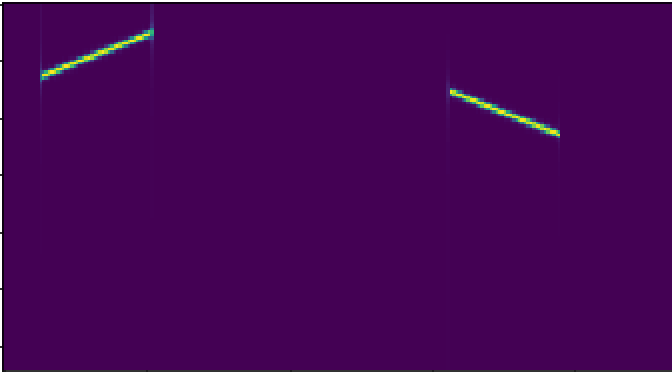
\includegraphics[width=3.0cm,height=3cm]{SpectrogramToy.png}
%\caption {\tiny{Example of spectrogram}}
\end{minipage}
\begin{minipage}[t]{3cm}
\centering
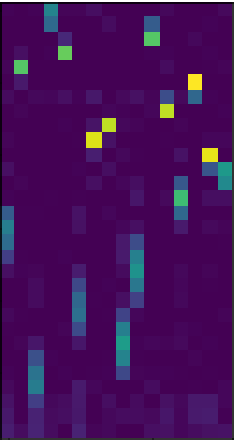
\includegraphics[width =3.0cm,height=3cm]{SpectralDictionaryPaper1.png}
%\caption{\tiny{Example of dictionary inferred by ONTDL}}
\end{minipage}
\caption{left(Spectrogram),right(Example of dictionary atoms)}
\end{figure}
We notice that the temporal patterns increase the ability of the classifier to perform a better discrimination.
\subsection{Real Data: DCase 2013}
For this data set,we resize the initial spectrograms to $60\times60$ images by cubic interpolation and compare the performances for different numbers of dictionary atoms and get the following chart:

%\section{REFERENCES}
%\label{sec:refs}
% References should be produced using the bibtex program from suitable
% BiBTeX files (here: strings, refs, manuals). The IEEEbib.bst bibliography
% style file from IEEE produces unsorted bibliography list.
% -------------------------------------------------------------------------
% \bibliographystyle{IEEEbib}
% \bibliography{strings,refs}
%\bibliography{ICASSPBiblio}

%\bibliographystyle{plain}
%\bibliography{ICASSPBiblio}

%\printbibliography


\appendix
\begin{center}
    \LARGE 
    Appendix
\end{center}
\section{Property}
Let's consider three matrices $\A\in \mathbb{R}^{M\times N}$,$\B\in\mathbb{R}^{L\times N}$,$I\in \mathbb{R}^{K\times K}$ the identity matrix and two  vector $\x \in \mathbb{R}^{KM\times 1}$,$\y \in \mathbb{R}^{LK\times 1}$ the problem:
\\
$\min \|(I\otimes \A)g-x\|^{2}_{2}+\lambda_{1}\|(I\otimes\B)g-y\|^{2}_{2}+\lambda_{2}\|g\|_{1}$\\
w.r.t $\g\in\mathbb{R}^{KN\times I},\g\geq 0$.%\hyperref[Propertyproblem]{($\mathcal{P}$)}\\
This problem can be dealt with by resolving independant nonnegative least squares with Lasso penalty.\\
Proof:let's denote the objective function of the problem $\zeta(\g)$.
By noticing 
$I\otimes \A$ is a block diagonal matrix with A on the diagonal, we have:$$
\begin{aligned}
\zeta(\g)&=\sum^{K}_{k=1}\underbrace{\|\begin{bmatrix}
                    \A\\
                    \sqrt{\lambda_{1}}\B\\
\end{bmatrix}\widehat{\g_{k}}-\begin{bmatrix}
                    \widehat{\x_{k}}\\
                    \sqrt{\lambda_{1}}\widehat{\y_{k}}\\
\end{bmatrix}\|^{2}_{2}+\lambda_{2}\|\widehat{\g_{k}}\|_{1}}_{\zeta(\g_{k})}
\end{aligned}
$$ with $\widehat{\g_{k}}\in\mathbb{R}^{N\times1}$ being a vector derived from $\g$ (respectively $\x$) by staking the values $\left\{\g_{i}\right\}_{(k-1)N+1\leq i \leq kN}$,
$\widehat{\x_{k}}\in\mathbb{R}^{M\times1}$ derived from $\x$ by stacking the values$\left\{\x_{i}\right\}_{(k-1)M+1\leq i \leq kM}$
$\widehat{\y_{k}}\in\mathbb{R}^{L\times1}$ by stacking the values $\left\{\y_{i}\right\}_{(k-1)L+1\leq i \leq kL}$. If $\g_{k,s}$ is a solution of the problem $\min_{\g_{k}\geq 0}\zeta(\g_{k})$, it is easy to see that $\g_{s}=[\g_{1,s},.,\g_{K,s}]$ is a solution of the initial problem.
\section{Updates}
Let's denote $\tG_{k},\A^{(f)}_{k},\A^{(t)}_{k},\B^{(f)}_{k},\B^{(t)}_{k}$ the value of the variables at the $k^{th}$ iteration. Since the Frobenius norm of a tensor is equal to Euclidean norm of its vectorized form, we have:\\
$\tG_{k+1}\leftarrow argmin\|Vec(\tX)-(I\otimes A^{(f)}_{k}\otimes A^{(t)}_{k})Vec(\tG)\|^{2}_{2}+\\ \lambda_{info}\|Vec(\tC)-(I\otimes B^{(f)}_{k}\otimes B^{(t)}_{k})Vec(\tG)\|^{2}_{2}+\lambda_{g}\|Veg(\tG)\|_{1}$. This problem is dealt with by resolving K nonnegative linear regression problems with Lasso penalty which are performed by the tool made available by $\cite{scikitlearnLasso}$. The updates for the four remaining variables $\A^{(f)},\A^{(t)},\B^{(f)},\B^{(t)}$ are performed by Projected Gradient Descent.  
\newpage
\bibliographystyle{plain}
\bibliography{ICASSPBiblio}
 \end{document}